\documentclass[red]{beamer}

\mode<presentation>
{
  \usetheme{Antibes}
  \usecolortheme{dolphin}
  \setbeamertemplate{footline}[frame number]
}

\usepackage[english]{babel}
\usepackage{subfigure}
\usepackage{xunicode}
\usepackage{xltxtra}
\usepackage{fontspec}
\usepackage{wrapfig}
\usepackage{subfigure}
\setmainfont{Ubuntu}

\title
{Modeling Civil Violence
}

\author
{Jeroen Hofman}

\institute
{
 Department of Computational Science\\
 University of Amsterdam}

\pgfdeclareimage[height=0.8cm]{university-logo}{logo.png}
\logo{\pgfuseimage{university-logo}}

\begin{document}
\graphicspath{{/home/jhofman/Desktop/CSS/Figures/}}
\setbeamertemplate{navigation symbols}{}

\begin{frame}
  \titlepage
\end{frame}

\section{Introduction}

\begin{frame}{Paper}
  \begin{center}
  \Large{
  Modifications based on a paper by Epstein. \\
  \vspace{10pt}
  \emph{Modeling Civil Violence, A Computational Agent-Based Approach.} \\}
\vspace{10pt}
\small{2002, PNAS, Vol. 99, No. 3, 7243-7250.}
  \end{center}
\end{frame}

\begin{frame}{Progress}
  Results from the paper:
  \begin{itemize}
  \item
    Simple interaction rules between civilians and cops on a grid produces outbursts of civilian activity (rebeling).
  \item
    Results produced by the system are very sensitive to parameter changes, but only a few are considered in the paper.
  \end{itemize}

  Further work:
  \begin{itemize}
  \item
    Much effort has been made to make the agents intelligent and let them evolve.
  \item
    Based on Epsteins model the military developed MANA, a simple interface for battlefield tactics.
  \end{itemize}

  \let\thefootnote\relax\footnotetext{\tiny{H. Queck, \emph{Evolutionary Game Theoretic Approach for Modeling Civil Violence.}, 2009, Evolutionary Computation, Vol. 13, No. 4, 780-800}}
  \let\thefootnote\relax\footnotetext{\tiny{B. Klemens et al., \emph{Empirical Performance of a Decentralized Civil Violence Model.}, 2010, Center on Social and Economics Dynamics Working Paper No. 56}}
\end{frame}

\begin{frame}{Research Questions}
  \begin{itemize}
  \item
    What is the effect of the agents vision range on outburst behavior?
  \item
    What is the effect of different movement strategies on outburst behavior?
  \end{itemize}
\end{frame}

\section{The Model}

\begin{frame}{Agent Behaviour}
  Two types of agents:
  \begin{itemize}
  \item
    Cops, serving an unspecified regime, can arrest civilians.
  \item
    Civilians, oppressed by an unspecified regime, can be active (rebels) or inactive.
  \end{itemize}

  Each civilians has the properties:
  \begin{itemize}
  \item
    Hardship $H$: measure for the amount of 'suffering' civilians go through. Initially uniform randomly drawn for each agent.
  \item
    Legitimacy $L$: measure for the amount of central authority. Initially fixed for all civilians.
  \item
    Grievance $G$: $G = H(1 - L)$, the amount of grievance each civilian experiences.
  \item
    Risk Aversion $R$: the inclination of the civilian to take risk. Initially uniform randomly drawn for each civilian.
  \end{itemize}

\end{frame}

\begin{frame}{Agent Behaviour}
  \small{
  All agents have a vision range $v$, a square block of size $2v + 1$ with the agent position as center.

  \vspace{10pt}

  Each civilian estimates its probability of getting arrested by:\\
  \vspace{10pt}
  \begin{center}
  $P = 1 - \exp(-k \lfloor(C/A)_v\rfloor)$
  \end{center}
  \vspace{10pt}
  where $(C/A)_v$ is the ratio of cops to agents in the vision range, $k$ is a constant.

  \vspace{10pt}

  Use $P$ to define the net risk $N = RP$.

  \vspace{10pt}
  \textbf{Civilian Rule}: If $G - N > T$, become active, otherwise, be inactive.\\
  $T$ is some threshold value.
}
\end{frame}

\begin{frame}{Agent Behaviour}
  \textbf{Cop Rule}: Inspect all sites within $v$ and arrest a random active civilian.

  \vspace{10pt}

  Cops move to position of active civilian and jail them for a uniform random number between 1 and $maxJail$.\\
  During this period the civilian cannot perform any actions.

  \vspace{10pt}

  \textbf{Movement Rule}: Move to a random unoccupied spot in $v$.
\end{frame}

\begin{frame}{Algorithm}
  \begin{columns}
    \column{3.0in}
    Start with 2D grid of size $N$x$N$ with continuous boundary conditions.
    Place agents randomly on the grid, number of agents defined by density $\rho_{\text{civ}}$ and $\rho_{\text{cop}}$.

    Every iteration up to $maxIter$:
    \begin{itemize}
    \item
      Create a shuffled list of all agents.
    \item
      Go through the list one by one, apply the movement rule to each agent and then the cop or civilian rule.\\
      (Do not do anything when the civilian is jailed.)
    \end{itemize}

    A large number of parameters is fixed.

    \column{1.5in}

    \begin{table}[H]
      \centering
      \begin{tabular}{l | l}
        Parameter & Value \\
        \hline
        $N$ & 40 \\
        $\rho_{\text{civ}}$ & 0.70 \\
        $\rho_{\text{cop}} $ & 0.04 \\
        $L$ & 0.8 \\
        $T$ & 0.1 \\
        $maxJail$ & 15 \\
        $k$ & 2.3 \\
      \end{tabular}
      \label{tab:param}
    \end{table}
  \end{columns}

\end{frame}

\begin{frame}{Modifications}
  \begin{itemize}
  \item
    Vision Range $v$: (Epstein: $v = 7$)\\
    $ 3 \leq v \leq 9$
  \vspace{10pt}
  \item
    Movement Rules: (Epstein: Random movement)\\
    \vspace{10pt}
    Cop: \\
    If an active civilian is in $v$, arrest it directly instead of moving randomly first. \\
    \vspace{10pt}
    Civilian: \\
    If active, move to the quadrant in $v$ with the largest number of active civilians.
  \end{itemize}
\end{frame}

\section{Results}

\begin{frame}{Original}
  Results for $v = 6$ and random movement (i.e. Epsteins model.). \\
  Three possible macroscopic states (and mixed forms) occur.
  \vspace{10pt}
  \begin{center}
    MOVIE
  \end{center}

  \begin{figure}[H]
    \centering
    \subfigure{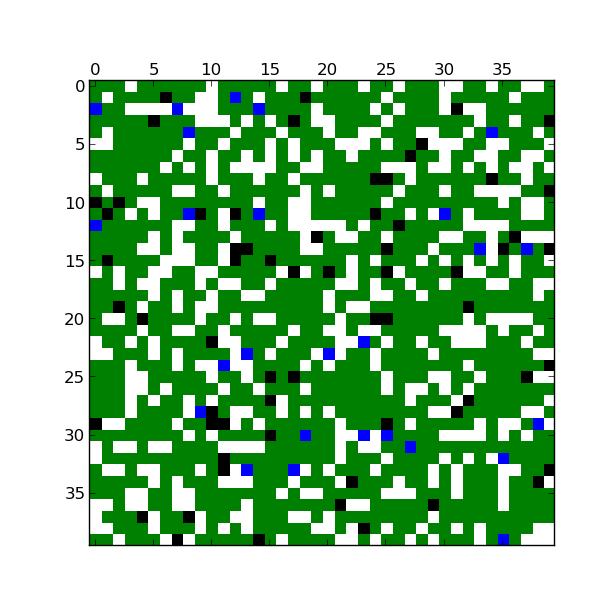
\includegraphics[width=0.3\textwidth]{state_1.png}}
    \subfigure{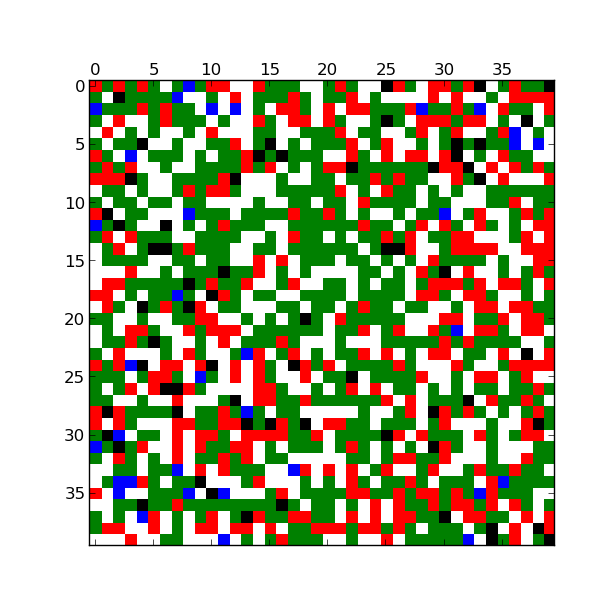
\includegraphics[width=0.3\textwidth]{state_2.png}}
    \subfigure{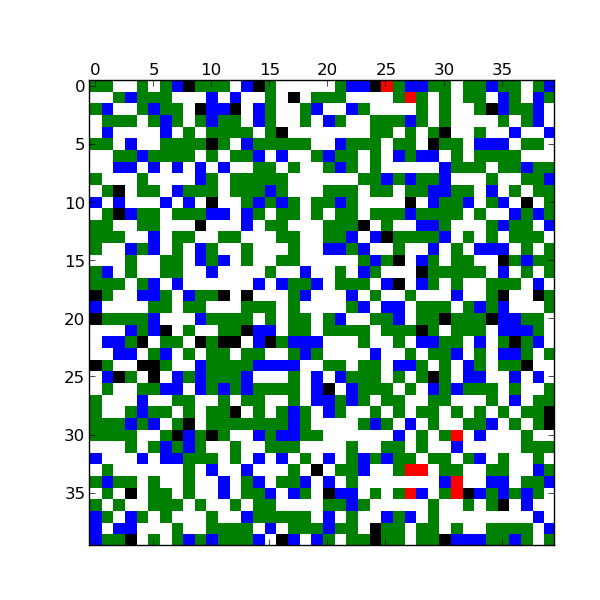
\includegraphics[width=0.3\textwidth]{state_3.png}}
    \label{fig:sample}
  \end{figure}
\end{frame}

\begin{frame}{Original}
  \begin{itemize}
  \item
    Outburst behavior is clearly visible.
  \item
    Peak in active civilians followed by peak in jailed civilians.
  \item
    Activity almost 0 between bursts, jailed agents on steady level.
  \item
    Maximum number of active agents around 400, caused by specific model parameters.
  \end{itemize}
  \begin{figure}[H]
    \centering
    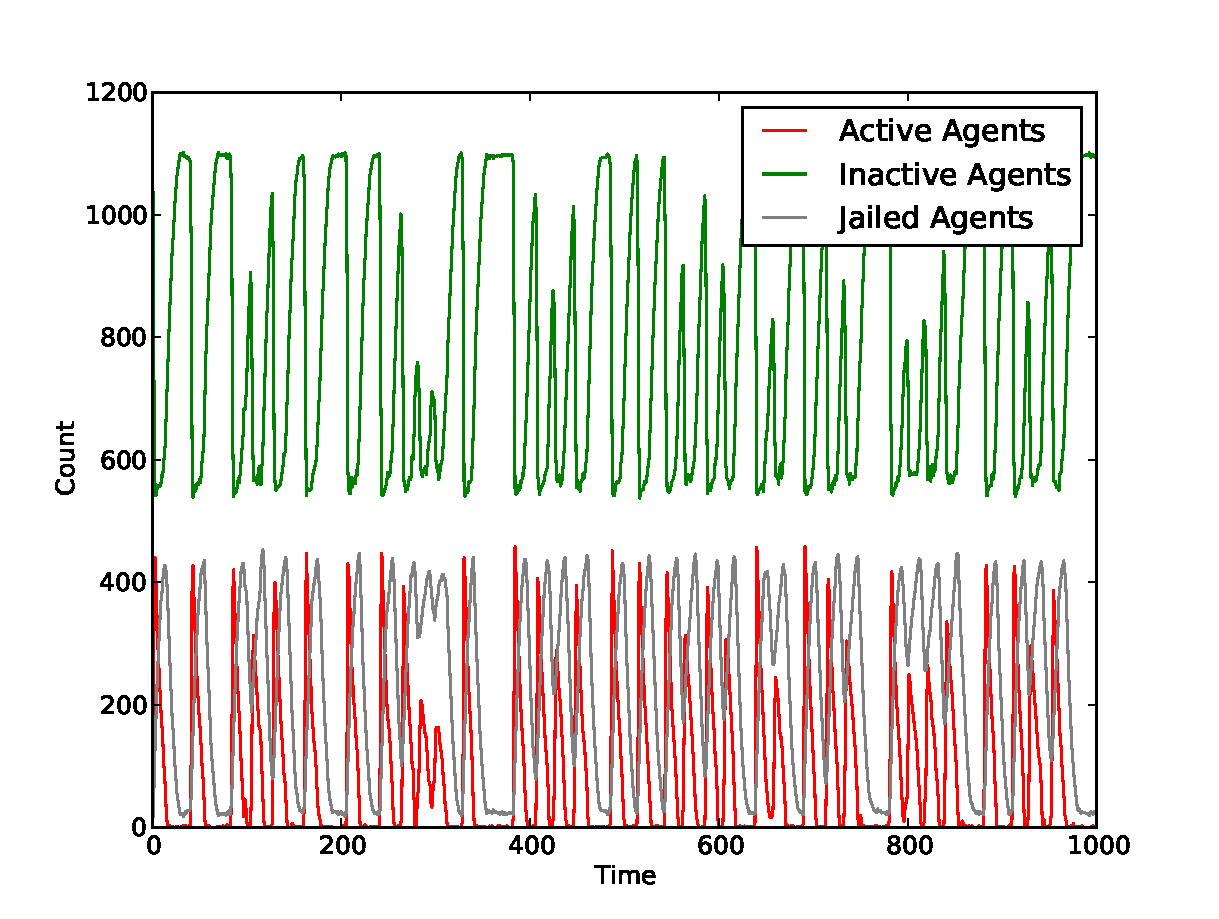
\includegraphics[width=0.6\textwidth]{original_sample.pdf}
    \label{fig:6}
  \end{figure}

\end{frame}

\begin{frame}{Vision Range}
  \begin{columns}
    \column{2.0in}
    Outburst behavior disappears, fluctuations around equilibrium value. \\
    Active regions cannot expand through the grid before they are 'killed' by cops due to low civilian vision range. \\
    Cops cannot see enough of the grid to be present in all places, constant number of small uprisings out of cop range.

    \column{2.5in}
    \begin{figure}[H]
      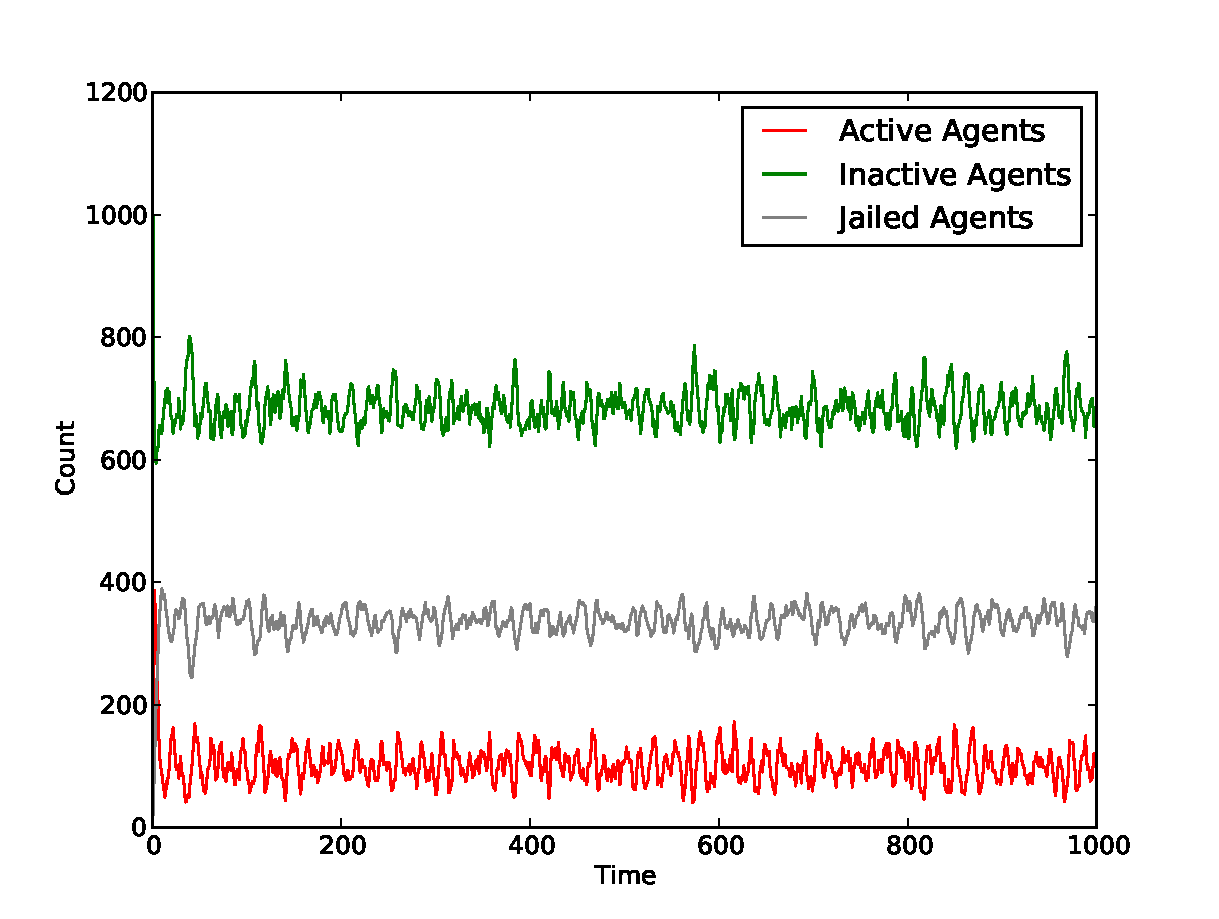
\includegraphics[width=2.5in]{original_3.pdf}
      \label{fig:3}
    \end{figure}
  \end{columns}
\end{frame}

\begin{frame}{Vision Range}

    \begin{table}[H]
      \footnotesize
      \centering
      \begin{tabular}{l | l}
        Vision Range & Number of outbursts \\
        \hline
        5 & 5316 \\
        6 & 2935 \\
        7 & 376
      \end{tabular}
      \label{tab:outburst}
    \end{table}

    \begin{itemize}
    \item
      If we set $v = 9$, we obtain 0 outbursts and almost 0 activity at all times, not very interesting.
    \item
      For intermediate values of $v$, i.e. 5, 6, 7 we observe a decrease in number of outbursts if $v$ increases.
    \item
      Note that the peak height does not depend on $v$.
    \end{itemize}
\end{frame}

\begin{frame}{Vision Range}

  \begin{figure}[H]
    \centering
    \subfigure{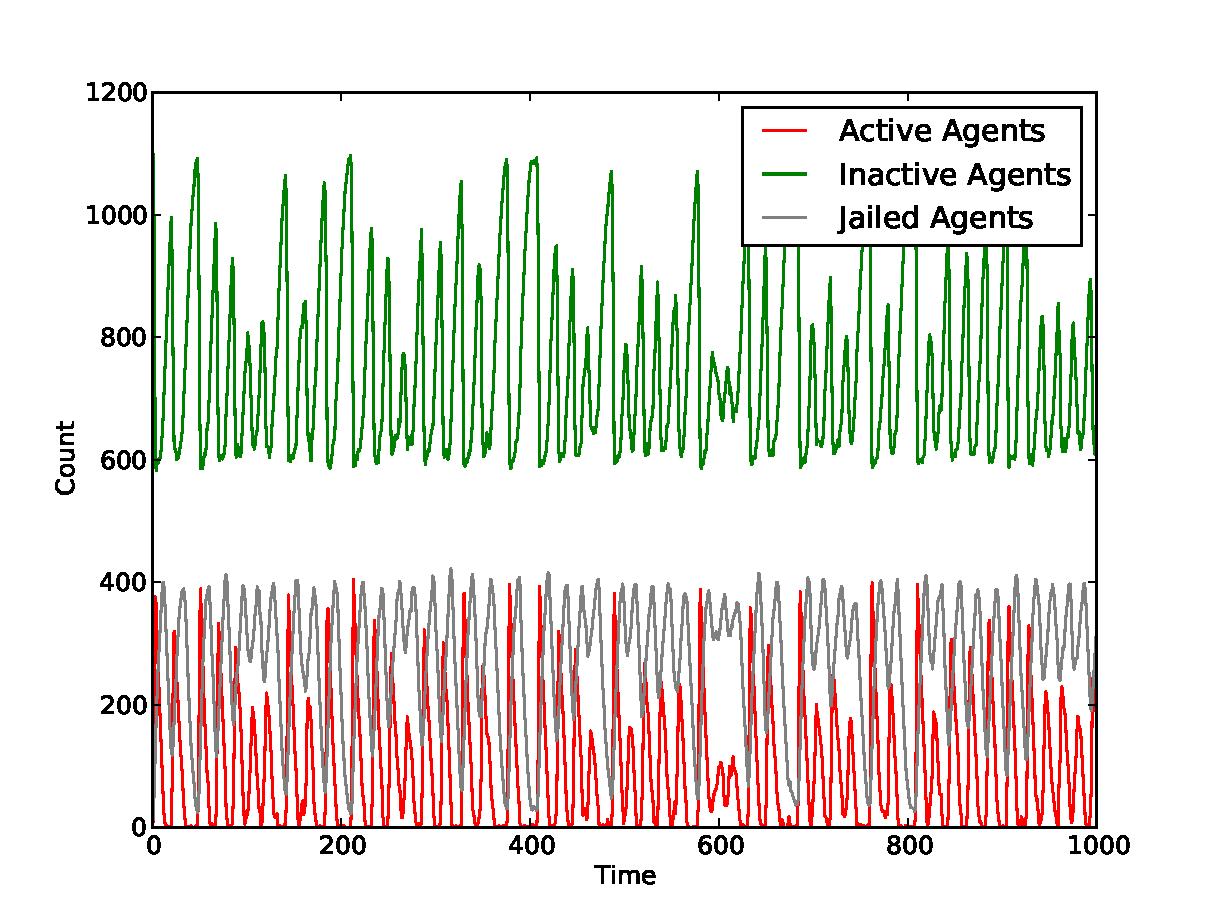
\includegraphics[width=0.43\textwidth]{original_5.pdf}}
    \subfigure{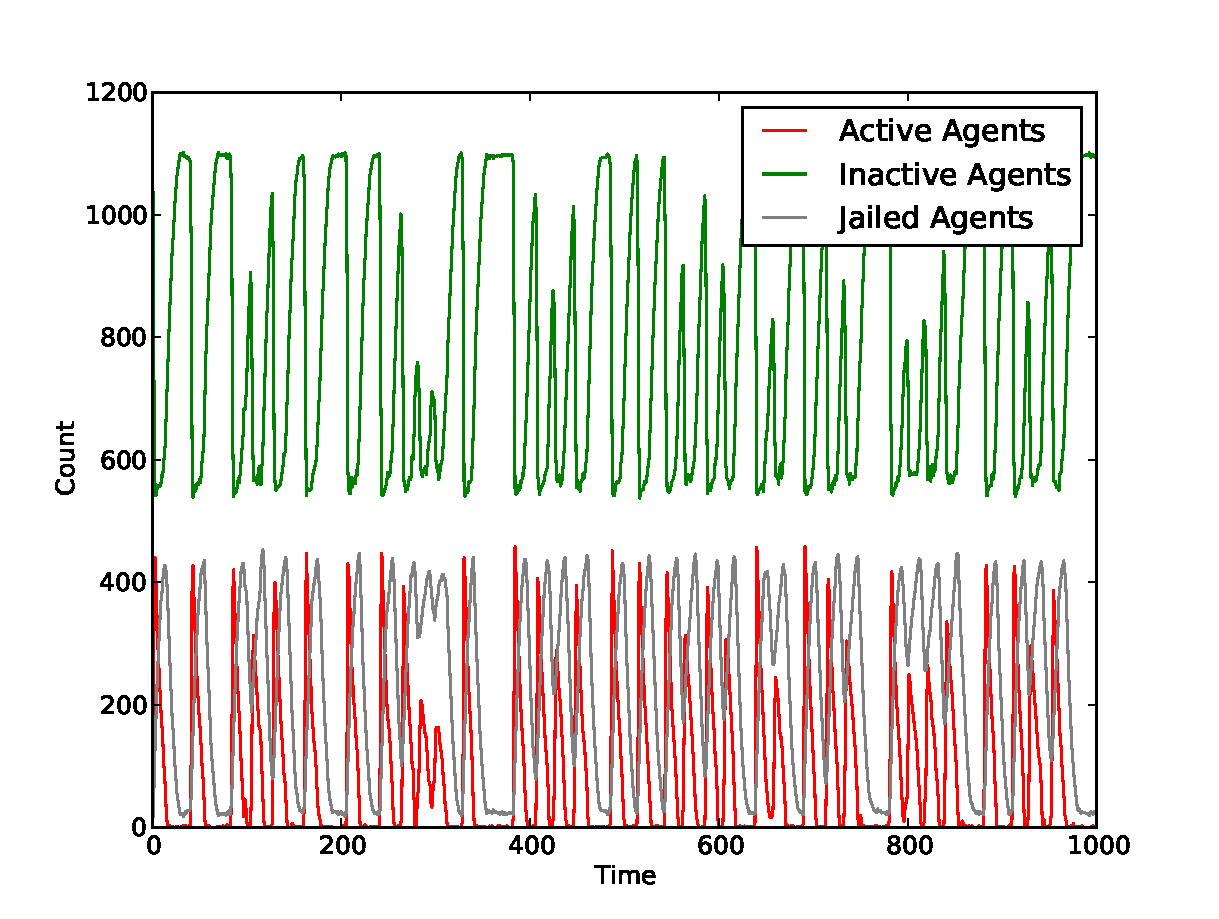
\includegraphics[width=0.43\textwidth]{original_sample.pdf}}
    \subfigure{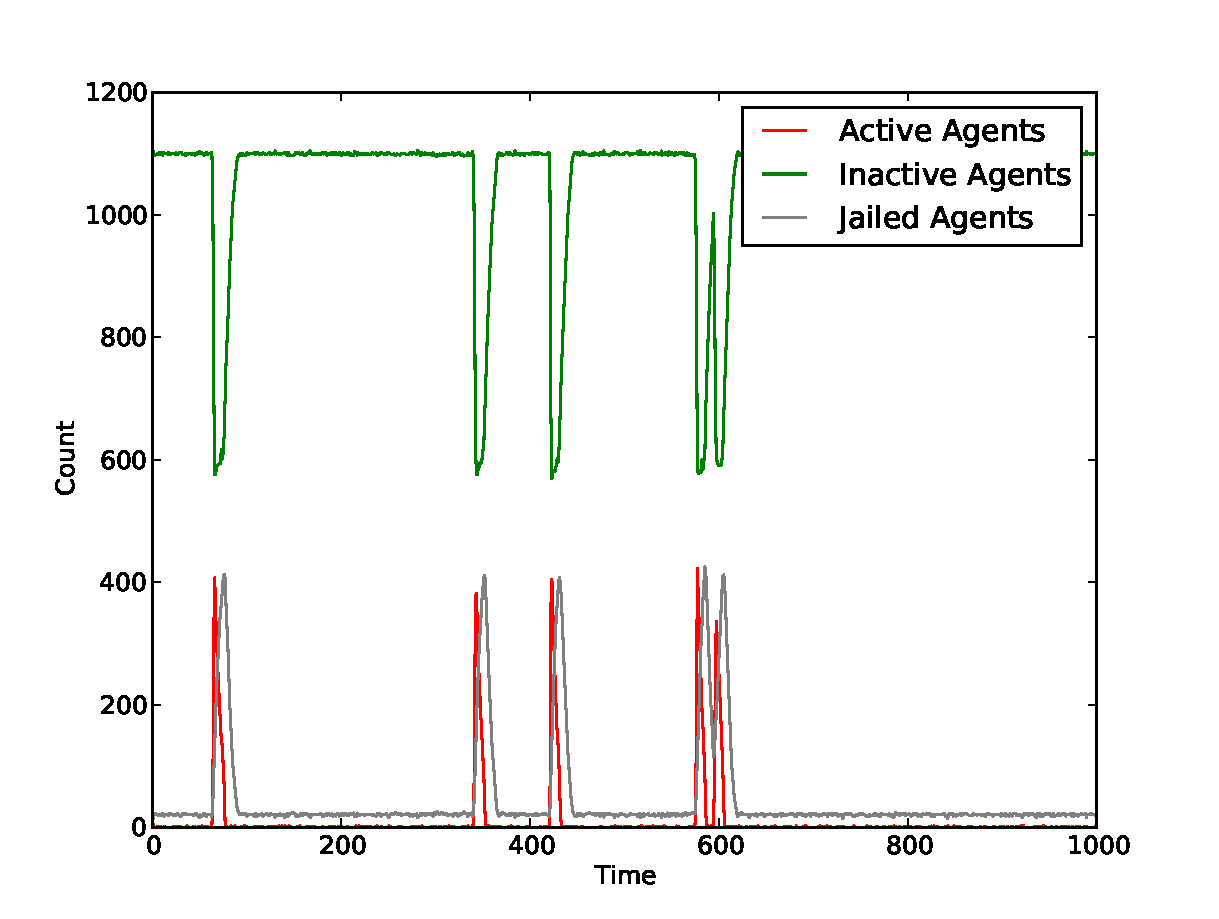
\includegraphics[width=0.43\textwidth]{original_7.pdf}}
    \label{fig:originals}
  \end{figure}

\end{frame}


\begin{frame}{Movement Strategies}
  \begin{itemize}
  \item
    Strategy I: The original random movements as implemented by Epstein.
  \item
    Strategy II: Active civilians move to the most 'active' quadrant.
  \item
    Strategy III: Cops can directly arrest an active civilian.
  \item
    Strategy IV: Strategy II + Strategy III
  \end{itemize}

\end{frame}

\begin{frame}{Movement Strategies}
  We introduce some additional statistics, example for strategy I ($v = 6$ , $10^5$ iterations):
  \begin{figure}[H]
    \centering
    \subfigure{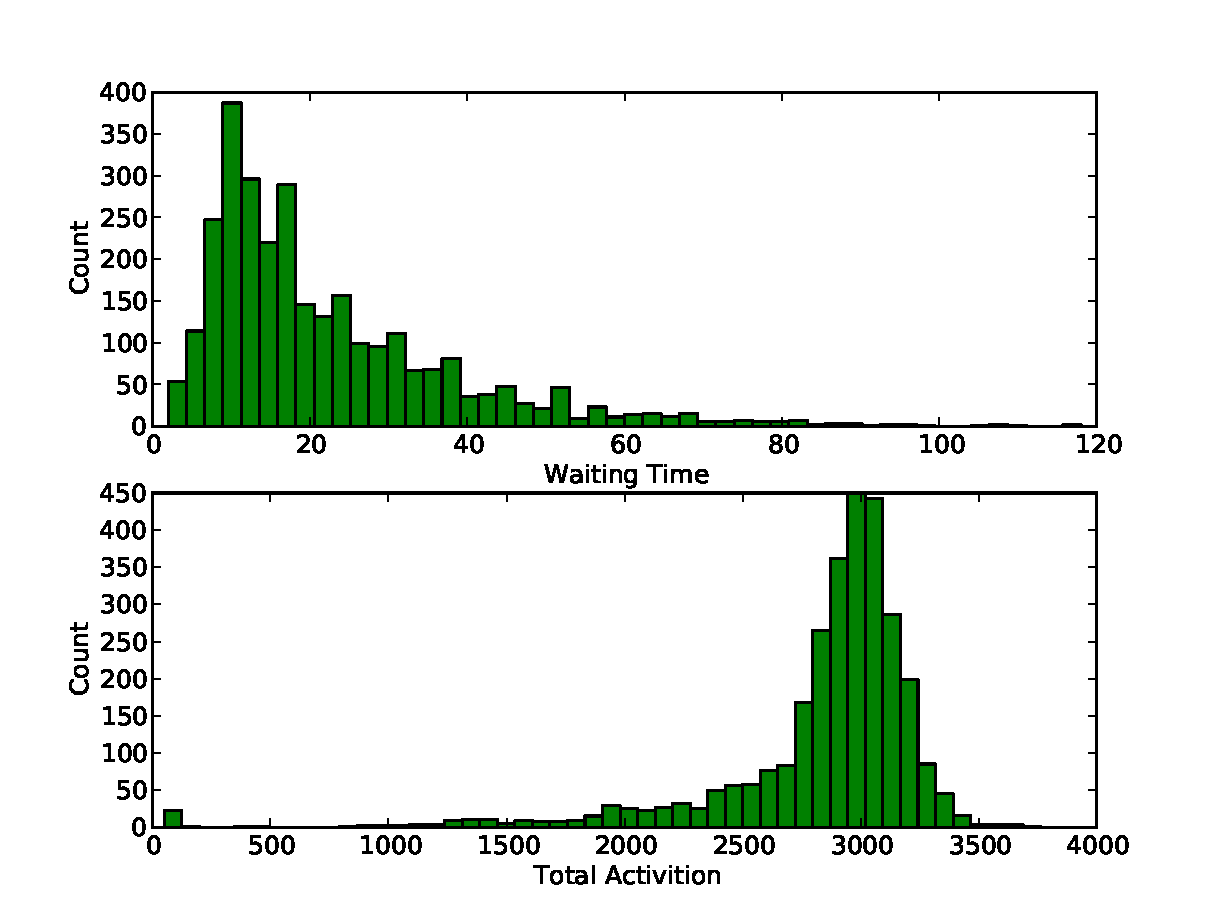
\includegraphics[width=0.43\textwidth]{original_dist.pdf}}
    \subfigure{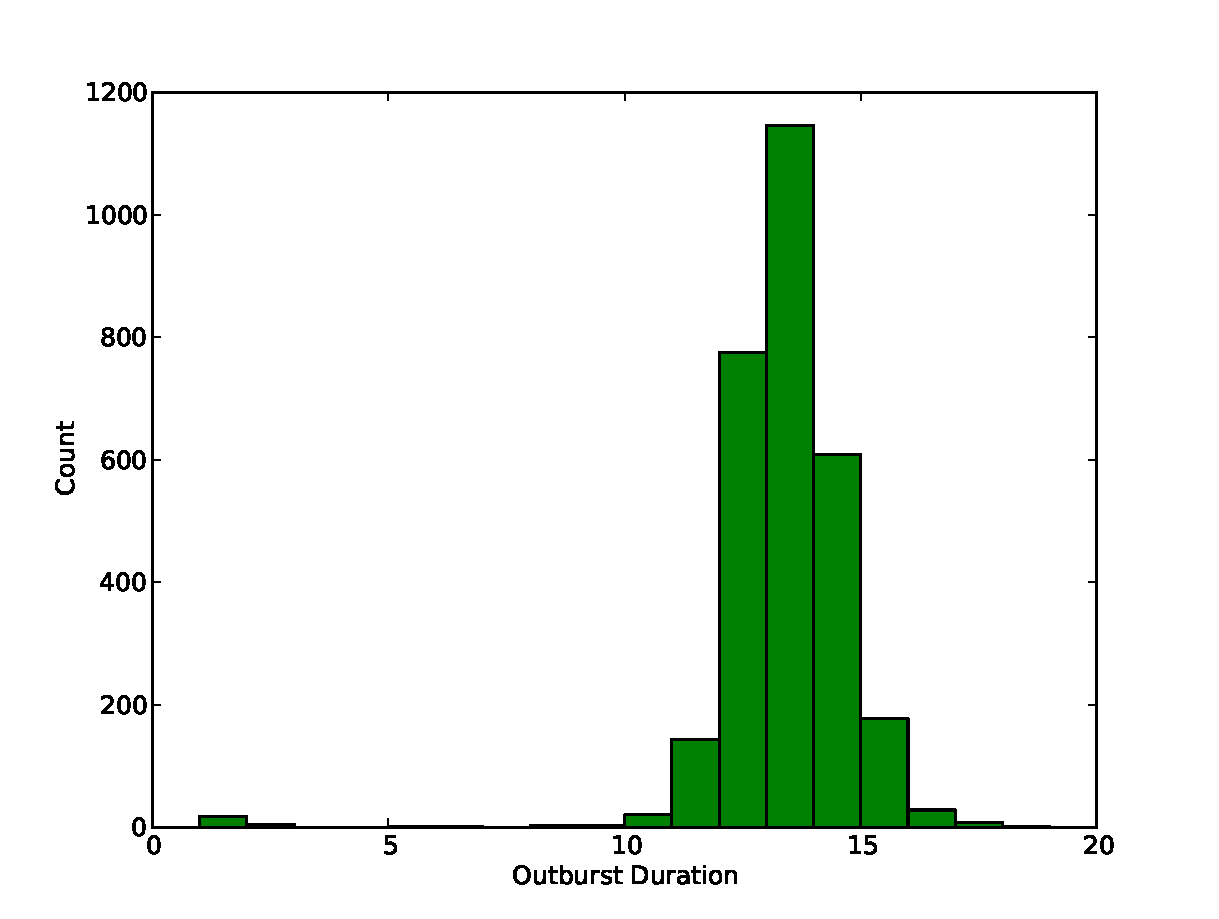
\includegraphics[width=0.43\textwidth]{original_outburst.pdf}}
    \label{fig:dist}
  \end{figure}

  Log-normal and normal distributions with outliers, use median for comparison.
\end{frame}

\begin{frame}{Movement Strategies}
  \begin{table}[H]
    \footnotesize
    \centering
    \begin{tabular}{c | c | c | c | c}
      Strategy & \# Outbursts & Med. Wait. Time & Med. Total Act. & Med. Outb. Dur. \\
      \hline
      I & 2935 & 17 & 2958 & 13 \\
      II & 3256 & 14 & 2559 & 12 \\
      III & 2629 & 30 & 2543 & 11 \\
      IV & 2057 & 30 & 1933 & 10
    \end{tabular}
    \label{tab:results}
  \end{table}
  Focus on Strategy I, II and III:\\
  \begin{itemize}
  \item
    Number of outbursts and waiting time behaves as expected.
  \item
    In strategy III total activation and outburst duration also behave as expected.
  \item
    Results are statistically different for waiting time (Mann-Whitney U test).
  \end{itemize}
  \let\thefootnote\relax\footnotetext{\tiny{H.B. Mann, D.R. Whitney \emph{On a Test of Whether one of Two Random Variables is Stochastically Larger than the Other.}, 1947, Annals of Mathematical Statistics, Vol. 18 No. 1, 50–60}}
\end{frame}

\begin{frame}{Movement Strategies}
  \begin{table}[H]
    \scriptsize
    \centering
    \begin{tabular}{c | c | c | c | c}
      Strategy & \# Outbursts & Med. Wait. Time & Med. Total Act. & Med. Outb. Dur. \\
      \hline
      I & 2935 & 17 & 2958 & 13 \\
      II & 3256 & 14 & 2559 & 12 \\
      III & 2629 & 30 & 2543 & 11 \\
      IV & 2057 & 30 & 1933 & 10
    \end{tabular}
    \label{tab:results}
  \end{table}
  \begin{columns}
    \column{2.0in}
    \begin{itemize}
    \item
      In strategy II behavior of total activation and outburst duration is unexpected.
    \item
      Caused by the addition of a lot of small outbursts.
    \item
      Distributions look similar between strategy I and III.
    \end{itemize}

    \column{2.5in}
    \begin{figure}[H]
      \centering
      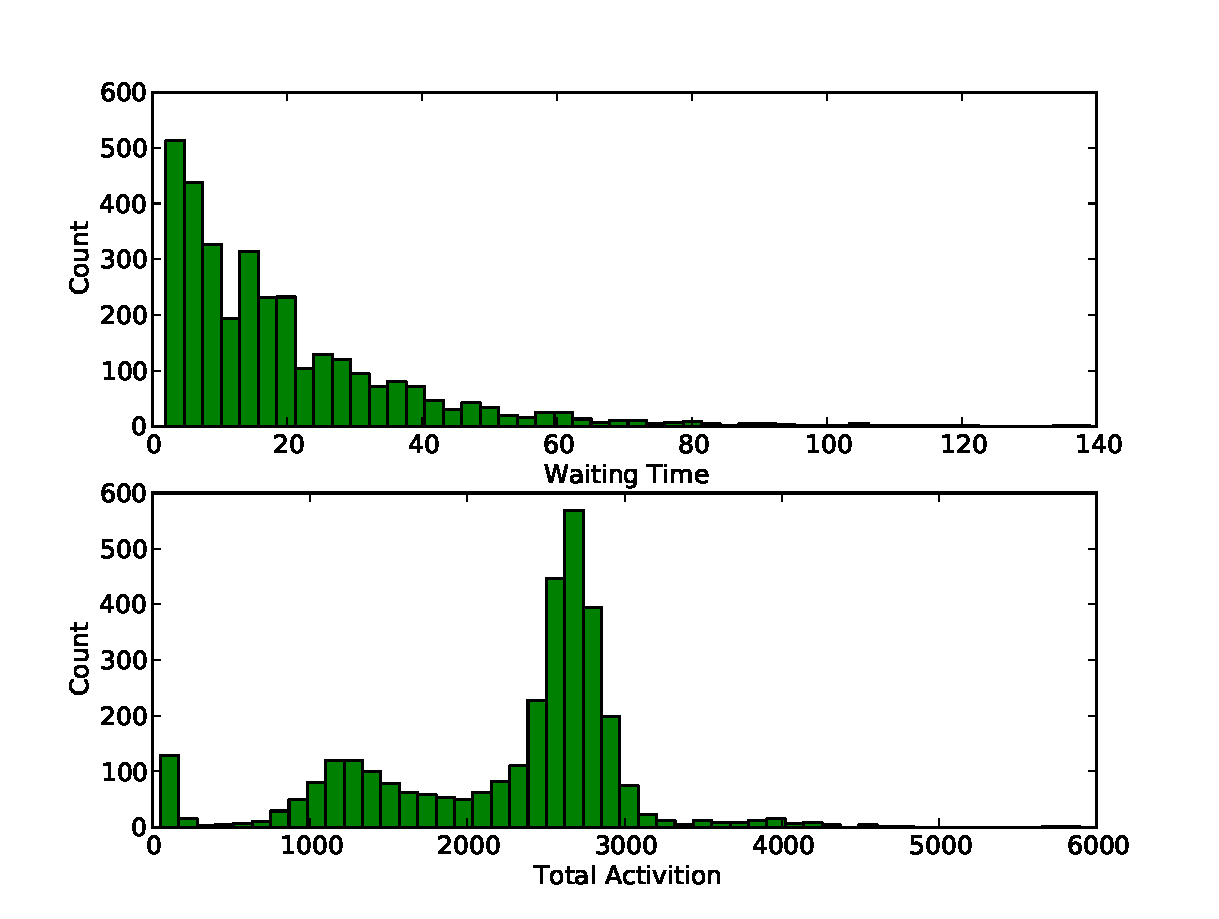
\includegraphics[width=2.5in]{moda_dist.pdf}
      \label{fig:strategy2}
    \end{figure}
  \end{columns}
\end{frame}

\begin{frame}{Movement Strategies}
  \begin{table}[H]
    \footnotesize
    \centering
    \begin{tabular}{c | c | c | c | c}
      Strategy & \# Outbursts & Med. Wait. Time & Med. Total Act. & Med. Outb. Dur. \\
      \hline
      I & 2935 & 17 & 2958 & 13 \\
      II & 3256 & 14 & 2559 & 12 \\
      III & 2629 & 30 & 2543 & 11 \\
      IV & 2057 & 30 & 1933 & 10
    \end{tabular}
    \label{tab:results}
  \end{table}
  \begin{itemize}
  \item
    Strategy IV shows that adding the two effects leads to increased suppression.
  \item
    Small number of outbursts, high waiting time (strategy III), small total and small outburst duration.
  \item
    Caused by herding of active civilians (strategy II) and the ability of cops to stay in the same area (strategy III).
  \item
    Cops move to area of high activity and stay there, while more actives are moving to that area because of high activity.
  \end{itemize}
\end{frame}

\section{Conclusion}
\begin{frame}{Conclusion}
  \begin{itemize}
  \item
    Different vision ranges produce different behavior, low values produce equilibrium values of activity, medium values produce outbursts and high values produce no activity.
  \item
    A slightly more intelligent movement strategy for the cops leads to decreased activity, for the civilians it leads to increased activity. Combined together it decreases activity, due to herding behaviour and the cops being able to stay in one area.
  \end{itemize}

  \vspace{15pt}
  \begin{center}
  \huge{Questions?}
  \end{center}
\end{frame}

\end{document}